\documentclass[aspectratio=169]{beamer}
%\documentclass{easytikz}


\usepackage{default}
\usepackage{tikz}
\usetikzlibrary{positioning,automata,calc}
\usepackage{multicol}


\usepackage{timing}

\usepackage[utf8]{inputenc}
\usepackage[T1]{fontenc}
\usepackage{minibox}
\usepackage{setspace}



\usetikzlibrary{shapes.geometric, arrows}
\usetikzlibrary{positioning}


\title{Programmierfallen -- unzulässige Kopplung}
\subtitle{\#1 unzulässige Kopplung von Zustand mit Programmablauf}
\author{Stefan Helmert}
\institute{entroserv.de}
\date{09/2019}

\logo{\Large\texttt{\minibox{entroserv\vspace{-.27cm}\\\hspace{0.63cm} course}}}

\tikzset{
  se/.style={rectangle, rounded corners, minimum width=3cm, minimum height=1cm,text centered, draw=black, fill=red!30},
  sed/.style={rectangle, rounded corners, minimum width=3cm, minimum height=1cm,text centered, draw=black, fill=black!30},
  io/.style={trapezium, trapezium left angle=70, trapezium right angle=110, minimum width=3cm, minimum height=1cm, text centered, draw=black, fill=blue!30},
  op/.style={rectangle, minimum width=3cm, minimum height=1cm, text centered, draw=black, fill=orange!30},
  cn/.style={diamond, minimum width=3cm, minimum height=1cm, text centered, draw=black, fill=green!30},
  sc/.style={circle, minimum width=2cm, minimum height=1cm, text centered, draw=black, fill=blue!30},
  node distance=7mm
}

\begin{document}
	
\frame{\titlepage}

\section{Ausgangssituation}
\subsection{Scheinbar nicht umsetzbar}
\begin{frame}[fragile]{\insertsection}{\insertsubsection}
\begin{multicols}{2}
	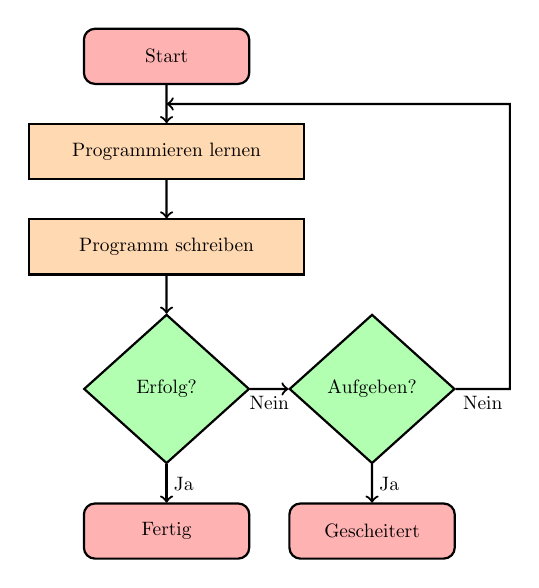
\begin{tikzpicture}[thick,scale=0.7, every node/.style={transform shape}]
	\node[se] (start) {Start};
	\node[op, below=of start, minimum width=5cm] (pl) {Programmieren lernen};
	\node[op, below=of pl, minimum width=5cm] (ps) {Programm schreiben};
	\node[cn, below=of ps, minimum height=2.7cm] (erfolg) {Erfolg?};
	\node[cn, right=of erfolg, minimum height=2.7cm] (aufgeben) {Aufgeben?};
	\node[se, below=of erfolg] (fertig) {Fertig};
	\node[se, below=of aufgeben] (gescheitert) {Gescheitert};	
	%
	\draw[->] (start) -- (pl) coordinate[midway] (startedge);

	\draw[->] (pl) -- (ps);
	\draw[->] (ps) -- (erfolg);
	\draw[->] (erfolg) -- node[right] {Ja} (fertig);
	\draw[->] (erfolg) -- node[below] {Nein}  (aufgeben);
	\draw[->] (aufgeben) -- node[right] {Ja} (gescheitert);
	\draw[->] (aufgeben) -- node[below] {Nein} ++(2.5,0) |- (startedge);
	\end{tikzpicture}
	\begin{itemize}
		\item Erlernen von Programmiersprachen
		\item Anschauen von Tutorials, Beispielen
		\item Beispielprogramme leicht umsetzbar
		\item reale Lösung nicht umsetzbar
	\end{itemize}

\end{multicols}
\end{frame}

\section{Problem}
\subsection{Vermeintlicher Konflikt}
\begin{frame}[fragile]{\insertsection}{\insertsubsection}
\begin{multicols}{2}
	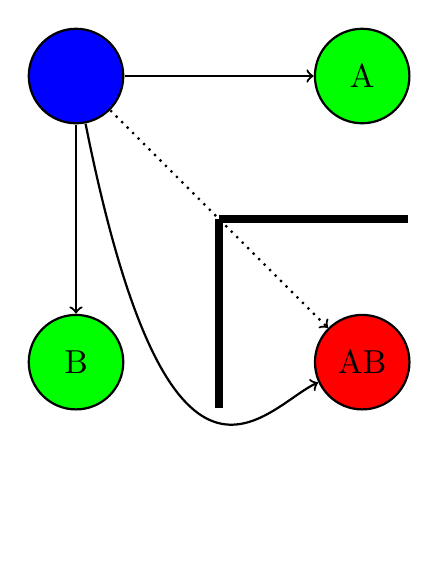
\begin{tikzpicture}[thick,scale=1.2, every node/.style={transform shape}, node distance=2cm, minimum width=1cm]
	\node[circle, draw=black, fill=blue] (start) {}; 
	\node[circle, draw=black, fill=green, right=of start] (A) {A};
	\node[circle, draw=black, fill=green, below=of start] (B) {B};
	\node[circle, draw=black, fill=red, below=of A] (AB) {AB};
	
	\draw[->] (start) -- (A);
	\draw[->] (start) -- (B);
	\draw[->,dotted] (start) -- (AB);
	\draw[->] (start) .. controls (1,-5) and (2,-3.5) .. (AB);
	\draw[line width=1mm] ($(start)!0.5!(AB)$) -- ++(2,0);
	\draw[line width=1mm] ($(start)!0.5!(AB)$) -- ++(0,-2);
	
	\end{tikzpicture}
	\begin{itemize}
		\item Anforderung A
		\begin{itemize}
			\item unmittelbar umsetzbar
		\end{itemize}
		\item Anforderung B
		\begin{itemize}
			\item unmittelbar umsetzbar
		\end{itemize}
		\item Kombination aus A, B
		\begin{itemize}
			\item komplexe Lösung
		\end{itemize}
		
	\end{itemize}
\end{multicols}
\end{frame}


\begin{frame}
	\tableofcontents
\end{frame}


\subsection{Anforderungsanalyse}
\begin{frame}[fragile]{\insertsection}{\insertsubsection}
\begin{multicols}{2}
	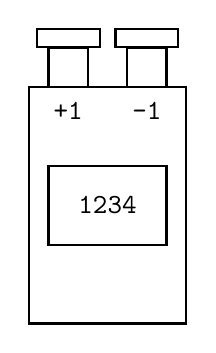
\begin{tikzpicture}[thick]
	\node[rectangle,draw=black,minimum width=0.8cm, minimum height=0.1cm] at (-0.5cm,2.125cm) {} ;
	\node[rectangle,draw=black,minimum width=0.5cm, minimum height=0.5cm] at (-0.5cm,1.75cm) {} ;
	\node[rectangle,draw=black,minimum width=0.8cm, minimum height=0.1cm] at (+0.5cm,2.125cm) {} ;
	\node[rectangle,draw=black,minimum width=0.5cm, minimum height=0.5cm] at (+0.5cm,1.75cm) {} ;
	\node[rectangle,minimum width=0.5cm, minimum height=0.5cm] at (+0.5cm,1.2cm) {\texttt{-1}} ;
	\node[rectangle,minimum width=0.5cm, minimum height=0.5cm] at (-0.5cm,1.2cm) {\texttt{+1}} ;
	\node[rectangle,draw=black,minimum width=1.5cm, minimum height=1cm] {};
	\node[rectangle,draw=black,minimum width=2cm, minimum height=3cm] {\texttt{1234}};
	\end{tikzpicture}\\
	
	\textbf{Aufgabe}
	\begin{itemize}
		\item zähle alle Tastendrücke
		\item Taste A erhöht um 1
		\item Taste B reduziert um 1
		\item nur ein Thread
		\item keine asynchrone Programmierung
	\end{itemize}

\end{multicols}
\end{frame}


\section{Problemanalyse}
\subsection{Nur Anforderung A}
\begin{frame}[fragile]{\insertsection}{\insertsubsection}
\begin{multicols}{2}
	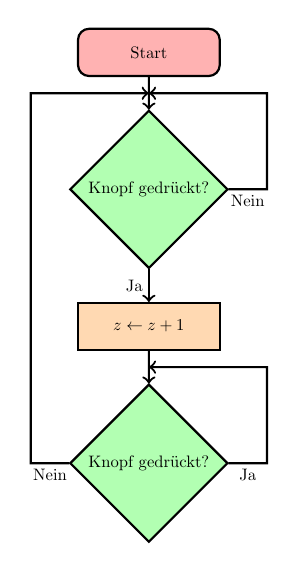
\begin{tikzpicture}[thick,scale=0.6, every node/.style={transform shape}]
	\node[se] (start) {Start};
	%\node[op, below=of div] (set) {$a=b,\ b=r$};
	\node[cn, below=of start] (condon) {Knopf gedrückt?};
	\node[op, below=of condon] (z) {$z \leftarrow z + 1$};
	\node[cn, below=of z] (condoff) {Knopf gedrückt?};
	
	%
	\draw[->] (start) -- (condon) coordinate[midway] (startedge);
	\draw[->] (condon) -- node[left] {Ja} (z);
	\draw[->] (z) -- (condoff) coordinate[midway] (condonedge);
	\draw[->] (condon) -- node[below] {Nein} ++(2.5,0) |- (startedge);
	\draw[->] (condoff) -- node[below] {Ja} ++(2.5,0) |- (condonedge);
	\draw[->] (condoff) -- node[below] {Nein} ++(-2.5,0) |- (startedge);
	\end{tikzpicture}
	\scalebox{0.7}{
		\begin{wave}{2}{5}
			\nextwave{Knopf} \bit{0}{1.0} \bit{1}{0.5} \bit{0}{0.5} \bit{1}{0.5} \bit{0}{0.5} \bit{1}{0.7} \bit{0}{.8} \bit{1}{1.7}
			\nextwave{$z$}  \known{0}{1.2} \known{1}{1} \known{2}{1} \known{3}{1.5} \known{4}{1.5}
		\end{wave}
	}
	\begin{itemize}
		\item zählt Tastendrücke: $z$
	\end{itemize}
\end{multicols}
\end{frame}


\begin{frame}[fragile]{\insertsection}{\insertsubsection}
\begin{multicols}{2}
	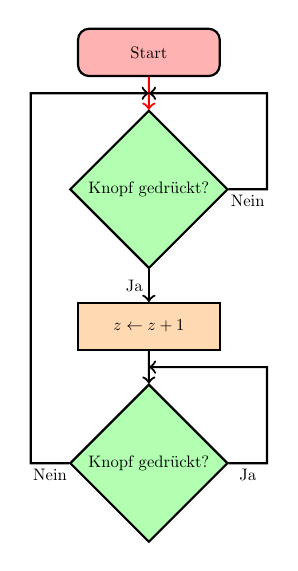
\begin{tikzpicture}[thick,scale=0.6, every node/.style={transform shape}]
	\node[se] (start) {Start};
	%\node[op, below=of div] (set) {$a=b,\ b=r$};
	\node[cn, below=of start] (condon) {Knopf gedrückt?};
	\node[op, below=of condon] (z) {$z \leftarrow z + 1$};
	\node[cn, below=of z] (condoff) {Knopf gedrückt?};
		%
	\draw[red,->] (start) -- (condon) coordinate[midway] (startedge);
	\draw[->] (condon) -- node[left] {Ja} (z);
	\draw[->] (z) -- (condoff) coordinate[midway] (condonedge);
	\draw[->] (condon) -- node[below] {Nein} ++(2.5,0) |- (startedge);
	\draw[->] (condoff) -- node[below] {Ja} ++(2.5,0) |- (condonedge);
	\draw[->] (condoff) -- node[below] {Nein} ++(-2.5,0) |- (startedge);
	\end{tikzpicture}
	\scalebox{0.7}{
		\begin{wave}{2}{5}
			\nextwave{Knopf} \bit{0}{1.0} \bit{1}{0.5} \bit{0}{0.5} \bit{1}{0.5} \bit{0}{0.5} \bit{1}{0.7} \bit{0}{.8} \bit{1}{1.7}
			\nextwave{$z$}  \known{0}{1.2} \known{1}{1} \known{2}{1} \known{3}{1.5} \known{4}{1.5}
			\nextwave{Zustand}  \ptr{0}{0} 
		\end{wave}
	}
	\begin{itemize}
		\item Knopf ist nicht gedrückt
		\item Programmstart
	\end{itemize}

\end{multicols}
\end{frame}



\begin{frame}[fragile]{\insertsection}{\insertsubsection}
\begin{multicols}{2}
	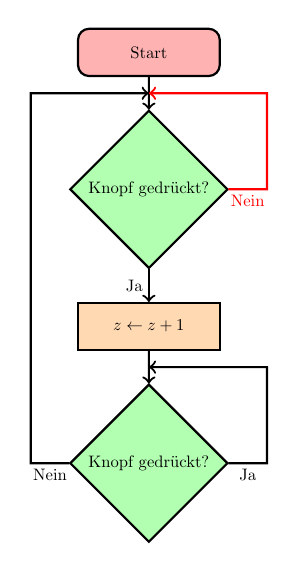
\begin{tikzpicture}[thick,scale=0.6, every node/.style={transform shape}]
	\node[se] (start) {Start};
	%\node[op, below=of div] (set) {$a=b,\ b=r$};
	\node[cn, below=of start] (condon) {Knopf gedrückt?};
	\node[op, below=of condon] (z) {$z \leftarrow z + 1$};
	\node[cn, below=of z] (condoff) {Knopf gedrückt?};
	%
	\draw[->] (start) -- (condon) coordinate[midway] (startedge);
	\draw[->] (condon) -- node[left] {Ja} (z);
	\draw[->] (z) -- (condoff) coordinate[midway] (condonedge);
	\draw[red,->] (condon) -- node[below] {Nein} ++(2.5,0) |- (startedge);
	\draw[->] (condoff) -- node[below] {Ja} ++(2.5,0) |- (condonedge);
	\draw[->] (condoff) -- node[below] {Nein} ++(-2.5,0) |- (startedge);
	\end{tikzpicture}
	\scalebox{0.7}{
		\begin{wave}{2}{5}
			\nextwave{Knopf} \bitr{0}{1.0} \bit{1}{0.5} \bit{0}{0.5} \bit{1}{0.5} \bit{0}{0.5} \bit{1}{0.7} \bit{0}{.8} \bit{1}{1.7}
			\nextwave{$z$}  \knownr{0}{1.2} \known{1}{1} \known{2}{1} \known{3}{1.5} \known{4}{1.5}
			\nextwave{Zustand}  \ptr{0}{0.5} 
		\end{wave}
	}
	\begin{itemize}
	\item Knopf ist nicht gedrückt
	\item Warteschleife solange Knopf nicht gedrückt ist
	\end{itemize}
\end{multicols}
\end{frame}

\begin{frame}[fragile]{\insertsection}{\insertsubsection}
\begin{multicols}{2}
	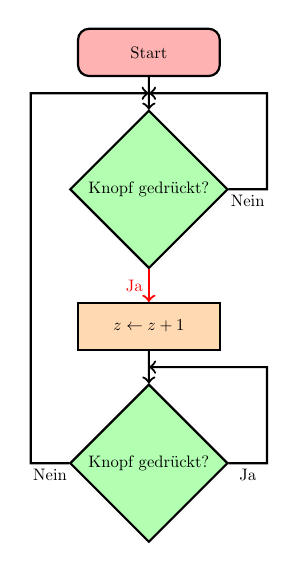
\begin{tikzpicture}[thick,scale=0.6, every node/.style={transform shape}]
	\node[se] (start) {Start};
	%\node[op, below=of div] (set) {$a=b,\ b=r$};
	\node[cn, below=of start] (condon) {Knopf gedrückt?};
	\node[op, below=of condon] (z) {$z \leftarrow z + 1$};
	\node[cn, below=of z] (condoff) {Knopf gedrückt?};
	%
	\draw[->] (start) -- (condon) coordinate[midway] (startedge);
	\draw[red,->] (condon) -- node[left] {Ja} (z);
	\draw[->] (z) -- (condoff) coordinate[midway] (condonedge);
	\draw[->] (condon) -- node[below] {Nein} ++(2.5,0) |- (startedge);
	\draw[->] (condoff) -- node[below] {Ja} ++(2.5,0) |- (condonedge);
	\draw[->] (condoff) -- node[below] {Nein} ++(-2.5,0) |- (startedge);
	\end{tikzpicture}
	\scalebox{0.7}{
		\begin{wave}{2}{5}
			\nextwave{Knopf} \bit{0}{1.0} \bitr{1}{0.5} \bit{0}{0.5} \bit{1}{0.5} \bit{0}{0.5} \bit{1}{0.7} \bit{0}{.8} \bit{1}{1.7}
			\nextwave{$z$}  \knownr{0}{1.2} \known{1}{1} \known{2}{1} \known{3}{1.5} \known{4}{1.5}
			\nextwave{Zustand}  \ptr{0}{1.0} 
		\end{wave}
	}
	\begin{itemize}
	\item Knopf ist gedrückt
	\item Warteschleife wird verlassen
	\end{itemize}
\end{multicols}
\end{frame}


\begin{frame}[fragile]{\insertsection}{\insertsubsection}
\begin{multicols}{2}
	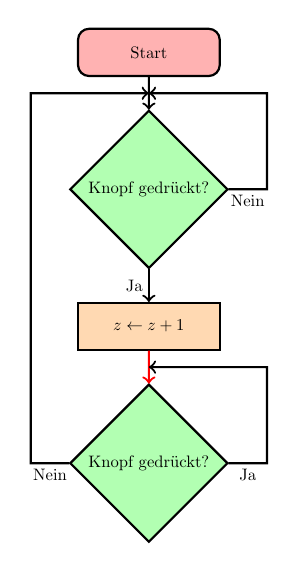
\begin{tikzpicture}[thick,scale=0.6, every node/.style={transform shape}]
	\node[se] (start) {Start};
	%\node[op, below=of div] (set) {$a=b,\ b=r$};
	\node[cn, below=of start] (condon) {Knopf gedrückt?};
	\node[op, below=of condon] (z) {$z \leftarrow z + 1$};
	\node[cn, below=of z] (condoff) {Knopf gedrückt?};
	%
	\draw[->] (start) -- (condon) coordinate[midway] (startedge);
	\draw[->] (condon) -- node[left] {Ja} (z);
	\draw[red,->] (z) -- (condoff) coordinate[midway] (condonedge);
	\draw[->] (condon) -- node[below] {Nein} ++(2.5,0) |- (startedge);
	\draw[->] (condoff) -- node[below] {Ja} ++(2.5,0) |- (condonedge);
	\draw[->] (condoff) -- node[below] {Nein} ++(-2.5,0) |- (startedge);
	\end{tikzpicture}
	\scalebox{0.7}{
		\begin{wave}{2}{5}
			\nextwave{Knopf} \bit{0}{1.0} \bitr{1}{0.5} \bit{0}{0.5} \bit{1}{0.5} \bit{0}{0.5} \bit{1}{0.7} \bit{0}{.8} \bit{1}{1.7}
			\nextwave{$z$}  \known{0}{1.2} \knownr{1}{1} \known{2}{1} \known{3}{1.5} \known{4}{1.5}
			\nextwave{Zustand}  \ptr{0}{1.2} 
		\end{wave}
	}
	\begin{itemize}
	\item Zählvariable $z$ erhöht um 1
	\item Beginn der Warteschleife bis Knopf losgelassen
	\end{itemize}

\end{multicols}
\end{frame}

\begin{frame}[fragile]{\insertsection}{\insertsubsection}
\begin{multicols}{2}
	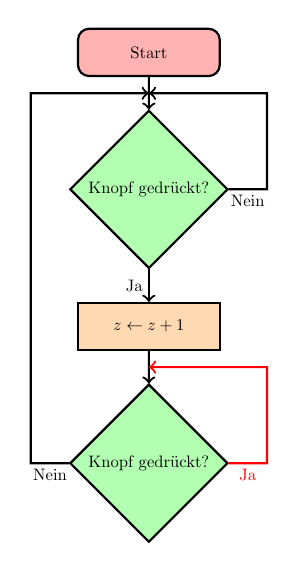
\begin{tikzpicture}[thick,scale=0.6, every node/.style={transform shape}]
	\node[se] (start) {Start};
	%\node[op, below=of div] (set) {$a=b,\ b=r$};
	\node[cn, below=of start] (condon) {Knopf gedrückt?};
	\node[op, below=of condon] (z) {$z \leftarrow z + 1$};
	\node[cn, below=of z] (condoff) {Knopf gedrückt?};
	%
	\draw[->] (start) -- (condon) coordinate[midway] (startedge);
	\draw[->] (condon) -- node[left] {Ja} (z);
	\draw[->] (z) -- (condoff) coordinate[midway] (condonedge);
	\draw[->] (condon) -- node[below] {Nein} ++(2.5,0) |- (startedge);
	\draw[red,->] (condoff) -- node[below] {Ja} ++(2.5,0) |- (condonedge);
	\draw[->] (condoff) -- node[below] {Nein} ++(-2.5,0) |- (startedge);
	\end{tikzpicture}
	\scalebox{0.7}{
		\begin{wave}{2}{5}
			\nextwave{Knopf} \bit{0}{1.0} \bitr{1}{0.5} \bit{0}{0.5} \bit{1}{0.5} \bit{0}{0.5} \bit{1}{0.7} \bit{0}{.8} \bit{1}{1.7}
			\nextwave{$z$}  \known{0}{1.2} \knownr{1}{1} \known{2}{1} \known{3}{1.5} \known{4}{1.5}
			\nextwave{Zustand}  \ptr{0}{1.4} 
		\end{wave}
	}
	\begin{itemize}
	\item Warteschleife bis Knopf losgelassen
	\end{itemize}
\end{multicols}
\end{frame}

\begin{frame}[fragile]{\insertsection}{\insertsubsection}
\begin{multicols}{2}
	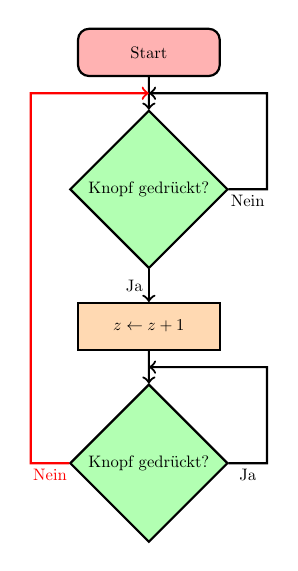
\begin{tikzpicture}[thick,scale=0.6, every node/.style={transform shape}]
	\node[se] (start) {Start};
	%\node[op, below=of div] (set) {$a=b,\ b=r$};
	\node[cn, below=of start] (condon) {Knopf gedrückt?};
	\node[op, below=of condon] (z) {$z \leftarrow z + 1$};
	\node[cn, below=of z] (condoff) {Knopf gedrückt?};
	%
	\draw[->] (start) -- (condon) coordinate[midway] (startedge);
	\draw[->] (condon) -- node[left] {Ja} (z);
	\draw[->] (z) -- (condoff) coordinate[midway] (condonedge);
	\draw[->] (condon) -- node[below] {Nein} ++(2.5,0) |- (startedge);
	\draw[->] (condoff) -- node[below] {Ja} ++(2.5,0) |- (condonedge);
	\draw[red,->] (condoff) -- node[below] {Nein} ++(-2.5,0) |- (startedge);
	\end{tikzpicture}
	\scalebox{0.7}{
		\begin{wave}{2}{5}
			\nextwave{Knopf} \bit{0}{1.0} \bit{1}{0.5} \bitr{0}{0.5} \bit{1}{0.5} \bit{0}{0.5} \bit{1}{0.7} \bit{0}{.8} \bit{1}{1.7}
			\nextwave{$z$}  \known{0}{1.2} \knownr{1}{1} \known{2}{1} \known{3}{1.5} \known{4}{1.5}
			\nextwave{Zustand}  \ptr{0}{1.5} 
		\end{wave}
	}
	\begin{itemize}
	\item Knopf losgelassen
	\item Warteschleife wird verlassen
	\item erneuter Aufruf der ersten Warteschleife
	\end{itemize}
\end{multicols}
\end{frame}

\begin{frame}[fragile]{\insertsection}{\insertsubsection}
\begin{multicols}{2}
	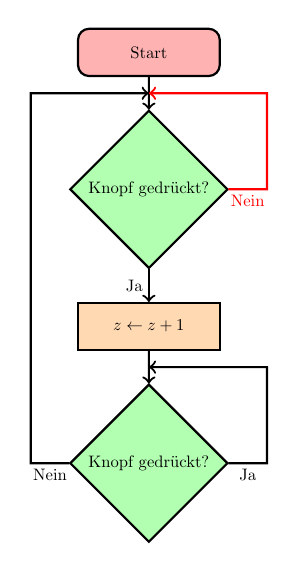
\begin{tikzpicture}[thick,scale=0.6, every node/.style={transform shape}]
	\node[se] (start) {Start};
	%\node[op, below=of div] (set) {$a=b,\ b=r$};
	\node[cn, below=of start] (condon) {Knopf gedrückt?};
	\node[op, below=of condon] (z) {$z \leftarrow z + 1$};
	\node[cn, below=of z] (condoff) {Knopf gedrückt?};
	%
	\draw[->] (start) -- (condon) coordinate[midway] (startedge);
	\draw[->] (condon) -- node[left] {Ja} (z);
	\draw[->] (z) -- (condoff) coordinate[midway] (condonedge);
	\draw[red,->] (condon) -- node[below] {Nein} ++(2.5,0) |- (startedge);
	\draw[->] (condoff) -- node[below] {Ja} ++(2.5,0) |- (condonedge);
	\draw[->] (condoff) -- node[below] {Nein} ++(-2.5,0) |- (startedge);
	\end{tikzpicture}
	\scalebox{0.7}{
		\begin{wave}{2}{5}
			\nextwave{Knopf} \bit{0}{1.0} \bit{1}{0.5} \bitr{0}{0.5} \bit{1}{0.5} \bit{0}{0.5} \bit{1}{0.7} \bit{0}{.8} \bit{1}{1.7}
			\nextwave{$z$}  \known{0}{1.2} \knownr{1}{1} \known{2}{1} \known{3}{1.5} \known{4}{1.5}
			\nextwave{Zustand}  \ptr{0}{1.7} 
		\end{wave}
	}
	\begin{itemize}
	\item Knopf nicht gedrückt
	\item Warteschleife bis Knopf gedrückt
	\end{itemize}
\end{multicols}
\end{frame}

\subsection{Beide Anforderungen A und B}
\begin{frame}[fragile]{\insertsection}{\insertsubsection}
\begin{multicols}{2}
	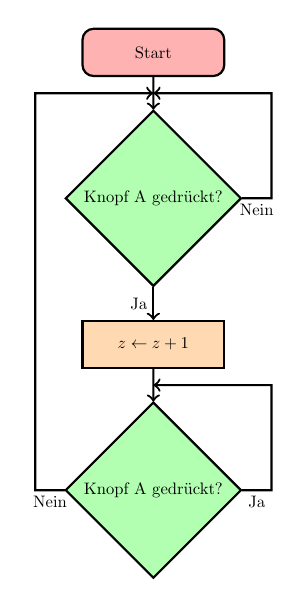
\begin{tikzpicture}[thick,scale=0.6, every node/.style={transform shape}]
	\node[se] (start) {Start};
	%\node[op, below=of div] (set) {$a=b,\ b=r$};
	\node[cn, below=of start] (condon) {Knopf A gedrückt?};
	\node[op, below=of condon] (z) {$z \leftarrow z + 1$};
	\node[cn, below=of z] (condoff) {Knopf A gedrückt?};
	%
	\draw[->] (start) -- (condon) coordinate[midway] (startedge);
	\draw[->] (condon) -- node[left] {Ja} (z);
	\draw[->] (z) -- (condoff) coordinate[midway] (condonedge);
	\draw[->] (condon) -- node[below] {Nein} ++(2.5,0) |- (startedge);
	\draw[->] (condoff) -- node[below] {Ja} ++(2.5,0) |- (condonedge);
	\draw[->] (condoff) -- node[below] {Nein} ++(-2.5,0) |- (startedge);
	\end{tikzpicture}
	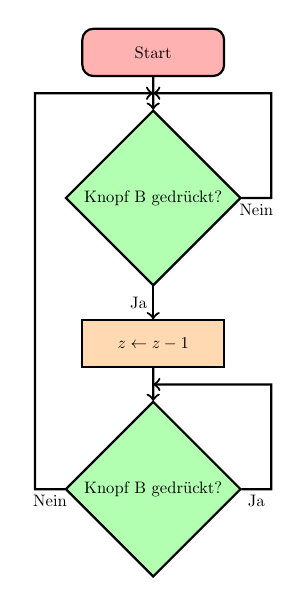
\begin{tikzpicture}[thick,scale=0.6, every node/.style={transform shape}]
	\node[se] (start) {Start};
	%\node[op, below=of div] (set) {$a=b,\ b=r$};
	\node[cn, below=of start] (condon) {Knopf B gedrückt?};
	\node[op, below=of condon] (z) {$z \leftarrow z - 1$};
	\node[cn, below=of z] (condoff) {Knopf B gedrückt?};
	%
	\draw[->] (start) -- (condon) coordinate[midway] (startedge);
	\draw[->] (condon) -- node[left] {Ja} (z);
	\draw[->] (z) -- (condoff) coordinate[midway] (condonedge);
	\draw[->] (condon) -- node[below] {Nein} ++(2.5,0) |- (startedge);
	\draw[->] (condoff) -- node[below] {Ja} ++(2.5,0) |- (condonedge);
	\draw[->] (condoff) -- node[below] {Nein} ++(-2.5,0) |- (startedge);
	\end{tikzpicture}
	\begin{itemize}
		\item Flussdiagramm duplizieren?
		\item aber Threads nicht erlaubt
	\end{itemize}
\end{multicols}
\end{frame}


\section{Lösungsansatz}
\subsection{Scheduling}
\begin{frame}[fragile]{\insertsection}{\insertsubsection}
\begin{multicols}{3}
	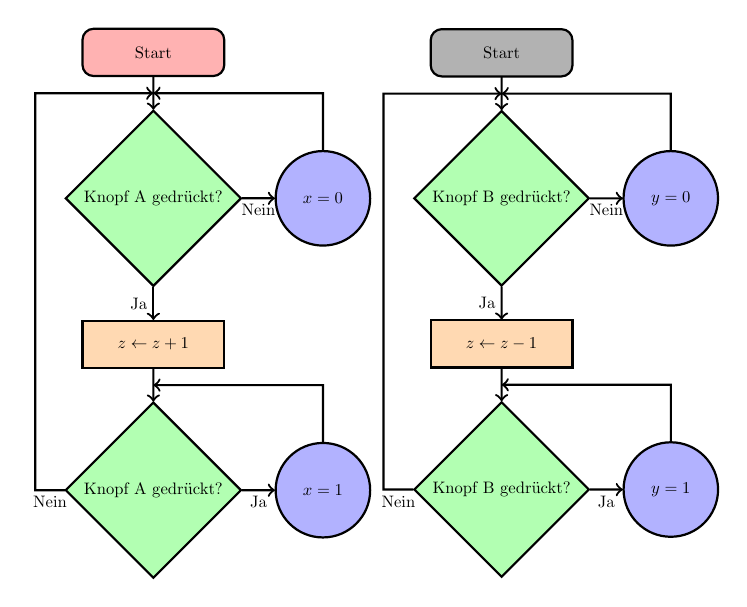
\begin{tikzpicture}[thick,scale=0.6, every node/.style={transform shape}]
	\node[se] (start) {Start};
	%\node[op, below=of div] (set) {$a=b,\ b=r$};
	\node[cn, below=of start] (condonA) {Knopf A gedrückt?};
	\node[op, below=of condonA] (zA) {$z \leftarrow z + 1$};
	\node[cn, below=of zA] (condoffA) {Knopf A gedrückt?};
	\node[sc, right=of condonA] (scA0) {$x=0$};
	\node[sc, right=of condoffA] (scA1) {$x=1$};
	%
	\draw[->] (start) -- (condonA) coordinate[midway] (startedge);
	\draw[->] (condonA) -- node[left] {Ja} (zA);
	\draw[->] (zA) -- (condoffA) coordinate[midway] (condonedgeA);
	\draw[->] (condonA) -- node[below] {Nein} (scA0);
	\draw[->] (scA0) -- node[below] {} ++(0,2.0) |- (startedge);
	\draw[->] (condoffA) -- node[below] {Ja} (scA1);
	\draw[->] (scA1) -- node[below] {} ++(0,2) |- (condonedgeA);
	\draw[->] (condoffA) -- node[below] {Nein} ++(-2.5,0) |- (startedge);

	%\node[op, below=of div] (set) {$a=b,\ b=r$};
	\node[right of=scA0, minimum width=1cm] (right) {};
	\node[cn, right=of right] (condonB) {Knopf B gedrückt?};
	\node[op, below=of condonB] (zB) {$z \leftarrow z - 1$};
	\node[cn, below=of zB] (condoffB) {Knopf B gedrückt?};
	\node[sc, right=of condonB] (scB0) {$y=0$};
	\node[sc, right=of condoffB] (scB1) {$y=1$};
	\node[sed, above=of condonB] (start) {Start};
	%
	\draw[->] (start) -- (condonB) coordinate[midway] (startedgeB);
	\draw[->] (condonB) -- node[left] {Ja} (zB);
	\draw[->] (zB) -- (condoffB) coordinate[midway] (condonedgeB);
	\draw[->] (scB0) -- node[below] {}  ++(0,2.0) |- (startedgeB);
	\draw[->] (condonB) -- node[below] {Nein}  (scB0);
	\draw[->] (condoffB) -- node[below] {Ja}  (scB1);
	\draw[->] (scB1) -- node[below] {} ++(0,2) |- (condonedgeB);
	\draw[->] (condoffB) -- node[below] {Nein} ++(-2.5,0) |- (startedgeB);
	\end{tikzpicture}
	\pagebreak
	\begin{itemize}
		\item implementiere Multithreading
		\item definiere Schedulingpunkt
		\item speichere Rücksprungpunkt
		\item Nachteile
		\begin{itemize}
			\item komplex
			\item fehleranfällig
		\end{itemize}
	\end{itemize}
\end{multicols}
\end{frame}

\subsection{Zustandsautomat}
\begin{frame}[fragile]{\insertsection}{\insertsubsection}
	\textbf{Zustandsautomat}
	\vspace{0.2cm}
	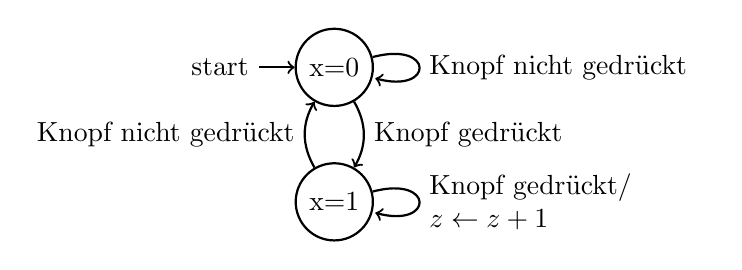
\begin{tikzpicture}[auto, thick]
	\node[initial,state] (q0) {x=0};
	\path
	(q0) edge[->, loop right] node {Knopf nicht gedrückt} ();
	\node[state, below=of q0] (q1) {x=1};
	\path
	(q0) edge[->, bend left] node {Knopf gedrückt} (q1)
	(q1) edge[->, loop right] node[text width=3.5cm,align=left] {Knopf gedrückt/\\ $z \leftarrow z + 1$} ()
	(q1) edge[->, bend left] node {Knopf nicht gedrückt} (q0);
	\end{tikzpicture}
	\begin{itemize}
		\item Betrachtung der Zustände
		\item Befehlsabfolge zunächst irrelevant
	\end{itemize}

\end{frame}


\begin{frame}[fragile]{\insertsection}{\insertsubsection}

\textbf{Zustandsautomat für Knopf A}

\vspace{0.2cm}

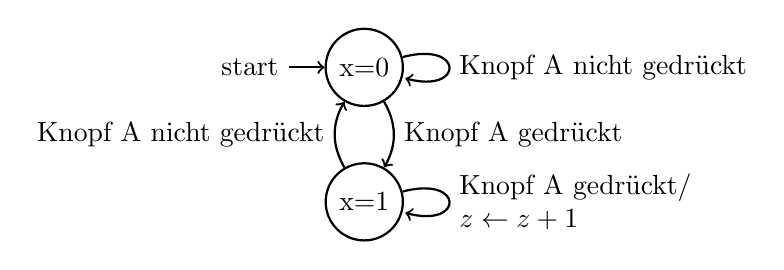
\begin{tikzpicture}[auto, thick]
\node[initial,state] (q0) {x=0};
\path
(q0) edge[->, loop right] node {Knopf A nicht gedrückt} ();
\node[state, below=of q0] (q1) {x=1};
\path
(q0) edge[->, bend left] node {Knopf A gedrückt} (q1)
(q1) edge[->, loop right] node[text width=3.5cm,align=left] {Knopf A gedrückt/\\ $z \leftarrow z + 1$} ()
(q1) edge[->, bend left] node {Knopf A nicht gedrückt} (q0);
\end{tikzpicture}

\vspace{0.4cm}

\textbf{Zustandsautomat für Knopf B}

\vspace{0.2cm}

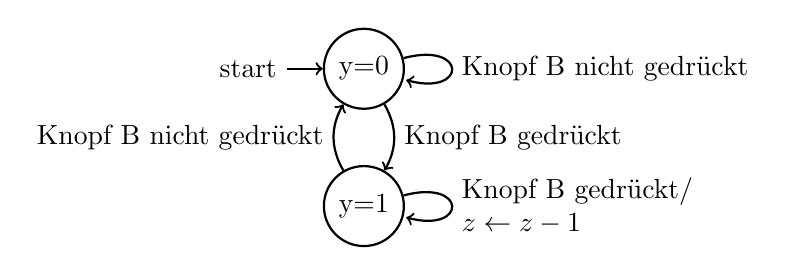
\begin{tikzpicture}[auto, thick]
\node[initial,state] (q0) {y=0};
\path
(q0) edge[->, loop right] node {Knopf B nicht gedrückt} ();
\node[state, below=of q0] (q1) {y=1};
\path
(q0) edge[->, bend left] node {Knopf B gedrückt} (q1)
(q1) edge[->, loop right] node[text width=3.5cm,align=left] {Knopf B gedrückt/\\ $z \leftarrow z - 1$} ()
(q1) edge[->, bend left] node {Knopf B nicht gedrückt} (q0);
\end{tikzpicture}


\end{frame}

\section{Lösung}
\subsection{Zustandsvariablen}
\begin{frame}[fragile]{\insertsection}{\insertsubsection}
\begin{multicols}{2}
	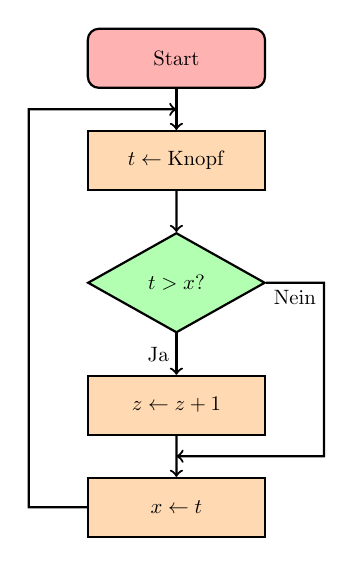
\begin{tikzpicture}[thick,scale=0.75, every node/.style={transform shape}]
	\node[se] (start) {Start};
	\node[op, below=of start] (tmp) {$t \leftarrow \mathrm{Knopf}$};
	\node[cn, below=of tmp] (condon) {$t > x?$};
	\node[op, below=of condon] (z) {$z \leftarrow z + 1$};
	\node[op, below=of z] (setx) {$x \leftarrow t$};
	%
	\draw[->] (start) -- (tmp) coordinate[midway] (startedge);
	\draw[->] (tmp) -- (condon);
	\draw[->] (condon) -- node[left] {Ja} (z);
	\draw[->] (z) -- (setx) coordinate[midway] (setxedge);
	\draw[->] (condon) -- node[below] {Nein} ++(2.5,0) |- (setxedge);
	\draw[->] (setx) -- ++(-2.5,0) |- (startedge);
	\end{tikzpicture}
	\begin{itemize}
		\item Zustand von Programmablauf getrennt
		\item Zustandsvariable $x$
		\item nur eine Hauptschleife
	\end{itemize}

\end{multicols}
\end{frame}

\begin{frame}[fragile]{\insertsection}{\insertsubsection}
\begin{multicols}{2}
	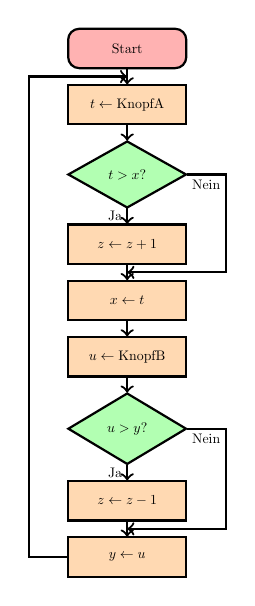
\begin{tikzpicture}[thick,scale=0.5, every node/.style={transform shape}, node distance=4mm]
	\node[se] (start) {Start};
	\node[op, below=of start] (tmpA) {$t \leftarrow \mathrm{KnopfA}$};

	
	\node[cn, below=of tmpA] (condonA) {$t > x?$};
	\node[op, below=of condonA] (zA) {$z \leftarrow z + 1$};
	
	\node[op, below=of zA] (setx) {$x \leftarrow t$};
	
	\node[op, below=of setx] (tmpB) {$u \leftarrow \mathrm{KnopfB}$};
	\node[cn, below=of tmpB] (condonB) {$u > y?$};
	\node[op, below=of condonB] (zB) {$z \leftarrow z - 1$};

	\node[op, below=of zB] (sety) {$y \leftarrow u$};
	%
	\draw[->] (start) -- (tmpA) coordinate[midway] (startedge);

	
	\draw[->] (tmpA) -- (condonA);
	
	\draw[->] (condonA) -- node[left] {Ja} (zA);
	\draw[->] (zA) -- (setx) coordinate[midway] (setxedge);
	\draw[->] (setx) -- (tmpB);
	\draw[->] (condonA) -- node[below] {Nein} ++(2.5,0) |- (setxedge);
	\draw[->] (tmpB) -- (condonB);

	\draw[->] (condonB) -- node[left] {Ja} (zB);
	\draw[->] (zB) -- (sety) coordinate[midway] (setyedge);
	\draw[->] (condonB) -- node[below] {Nein} ++(2.5,0) |- (setyedge);

	
	\draw[->] (sety) -- ++(-2.5,0) |- (startedge);
	\end{tikzpicture}
	\begin{itemize}
		\item erfolgreiche Kombination beider Anforderungen
		\item Zustand von Programmablauf getrennt
		\item Zustandsvariablen 
	\begin{itemize}
		\item $x$ für Knopf~A
		\item $y$ für Knopf~B
	\end{itemize}
		\item nur eine Hauptschleife
	\begin{itemize}
		\item nur ein Sprung zurück
	\end{itemize}
\end{itemize}	
\end{multicols}
\end{frame}

\begin{frame}[fragile]{\insertsection}{\insertsubsection}
\begin{multicols}{2}
	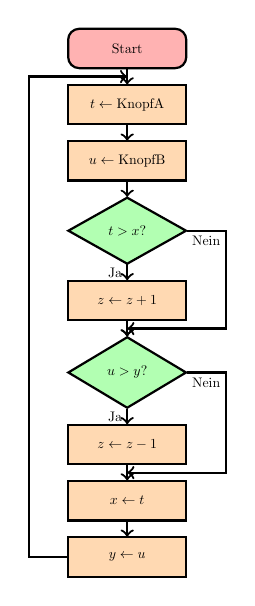
\begin{tikzpicture}[thick,scale=0.5, every node/.style={transform shape}, node distance=4mm]
	\node[se] (start) {Start};
	\node[op, below=of start] (tmpA) {$t \leftarrow \mathrm{KnopfA}$};
	\node[op, below=of tmpA] (tmpB) {$u \leftarrow \mathrm{KnopfB}$};
	
	\node[cn, below=of tmpB] (condonA) {$t > x?$};
	\node[op, below=of condonA] (zA) {$z \leftarrow z + 1$};
	

	
	\node[cn, below=of zA] (condonB) {$u > y?$};
	\node[op, below=of condonB] (zB) {$z \leftarrow z - 1$};

	\node[op, below=of zB] (setx) {$x \leftarrow t$};	
	\node[op, below=of setx] (sety) {$y \leftarrow u$};
	%
	\draw[->] (start) -- (tmpA) coordinate[midway] (startedge);
	\draw[->] (tmpA) -- (tmpB);
	
	\draw[->] (tmpB) -- (condonA);
	
	\draw[->] (condonA) -- node[left] {Ja} (zA);
	\draw[->] (zA) -- (condonB) coordinate[midway] (setxedge);
	\draw[->] (condonA) -- node[below] {Nein} ++(2.5,0) |- (setxedge);

	
	\draw[->] (zA) -- (condonB);
	\draw[->] (zB) -- (setx) coordinate[midway] (setyedge);
	\draw[->] (condonB) -- node[below] {Nein} ++(2.5,0) |- (setyedge);
	\draw[->] (condonB) -- node[left] {Ja} (zB);
		
	\draw[->] (setx) -- (sety);	
	\draw[->] (sety) -- ++(-2.5,0) |- (startedge);
	\end{tikzpicture}
	\begin{itemize}
		\item Umsortieren nach EVA-Prinzip
		\begin{itemize}
			\item Wartbarkeit
		\end{itemize}
	\end{itemize}	
\end{multicols}
\end{frame}

\section{Kontakt}
\begin{frame}[fragile]{\insertsection}{\insertsubsection}
\scalebox{1.2}{%
\begin{minipage}{2\textwidth}
	\begin{description}
		\item[Folien] \url{https://github.com/TheTesla/ProgrammierTutorial}
		\item[Github] \url{https://github.com/TheTesla}
		\item[Webseite] \url{https://entroserv.de/}
		\item[Mailingliste] \url{https://www.lists.entroserv.de/listinfo/lounge}
		\item[E-Mail] \href{mailto:stefan@entroserv.de}{stefan@entroserv.de}
		\item[Telegram] @Tesla423
	\end{description}
\end{minipage}%
}

\end{frame}

\end{document}
